% This is samplepaper.tex, a sample chapter demonstrating the
% LLNCS macro package for Springer Computer Science proceedings;
% Version 2.21 of 2022/01/12
%
\documentclass[runningheads]{llncs}
%
\usepackage[T1]{fontenc}
% T1 fonts will be used to generate the final print and online PDFs,
% so please use T1 fonts in your manuscript whenever possible.
% Other font encondings may result in incorrect characters.
%
\usepackage{graphicx}
\usepackage{acronym}
\usepackage[backend=biber,style=lncs]{biblatex}
\usepackage[inline]{enumitem}
\usepackage{cleveref}
% Used for displaying a sample figure. If possible, figure files should
% be included in EPS format.
%
% If you use the hyperref package, please uncomment the following two lines
% to display URLs in blue roman font according to Springer's eBook style:
%\usepackage{color}
%\renewcommand\UrlFont{\color{blue}\rmfamily}
%
\addbibresource{bibliography.bib}
\addbibresource{mypubblications.bib}

\acrodef{cas}[CAS]{Collective Adaptive Systems}
\acrodef{iot}[IoT]{Internet of Things}
\acrodef{ecc}[ECC]{Edge-Cloud Continuum}
\acrodef{rl}[RL]{Reinforcement Learning}
\acrodef{gnn}[GNN]{Graph Neural Networks}

\begin{document}

%
\title{{\normalfont PhD Thesis Proposal}\\\vspace{0.1em}Engineering Collective Systems in the Wearable Edge-Cloud Continuum: Models and Platforms
%\thanks{Supported by organization x.}
}
%
\titlerunning{PhD Thesis Proposal -- Cycle 39}
% If the paper title is too long for the running head, you can set
% an abbreviated paper title here
%
\author{Nicolas Farabegoli\inst{1}\orcidID{0000-0002-7321-358X}\\Cycle 39 -- Computer Science and Engineering} %\inst{1}\orcidID{0000-0002-7321-358X}}
%
%\authorrunning{F. Author et al.}
% First names are abbreviated in the running head.
% If there are more than two authors, 'et al.' is used.
%
\institute{
    Alma Mater Studiorum -- Università di Bologna, Cesena (FC) 47522, Italy
    \email{nicolas.farabegoli@unibo.it}
}
%
\maketitle              % typeset the header of the contribution
%
\begin{abstract}
% The abstract should briefly summarize the contents of the paper in
% 150--250 words.
The Edge-Cloud Continuum (ECC) has emerged as a solution to the limitations of traditional cloud systems by enabling a more flexible and scalable infrastructure that spans multiple computational tiers,
from IoT devices to the cloud.
%
Several approaches have been proposed to leverage the ECC in IoT applications and Collective Adaptive Systems (CAS);
however,
they are often tailored to specific use cases,
focusing on isolated aspects such as latency,
energy efficiency,
and system performance.
%
This makes them difficult to generalize and reuse across different contexts.
%
This PhD thesis aims to develop a general and comprehensive framework to support the design and deployment of the next generation of IoT and CAS in the ECC,
providing a general model specifically designed at the intersection of other research areas:
self-organisation principles for defining the collective and collaborative behavior of the system,
multi-tier programming models for handling the heterogeneity of the infrastructure producing sound system specifications,
and AI-driven techniques like reinforcement learning for dynamic resource management,
predictive scaling,
and dynamic system reconfiguration.

% \keywords{First keyword  \and Second keyword \and Another keyword.}
\end{abstract}

\section{Introduction}
\label{sec:introduction}
The rapid proliferation of interconnected devices in environments such as smart cities,
IoT ecosystems,
wearable devices,
and swarm robotics has introduced new challenges in system design and management.
%
These systems,
characterized by numerous devices with varying capabilities and constraints,
must interact cooperatively and adaptively in dynamic environments.
%
Traditional cloud-based solutions,
limited by latency and bandwidth constraints,
are increasingly being replaced by the \ac{ecc}~\cite{DBLP:journals/access/MoreschiniPLNHT22},
which enables distributed computing across multiple tiers.

This research aims to develop innovative approaches for engineering \ac{cas}~\cite{DBLP:conf/birthday/BucchiaroneM19} within the \ac{ecc}.
%
The proposed framework will support the entire \ac{cas} workflow,
from design and deployment to runtime management and adaptation.
%
By leveraging self-organization principles,
the framework will ensure coherent collective behavior,
while multitier~\cite{DBLP:journals/csur/WeisenburgerWS20} programming models will address the heterogeneity and layered characteristics of modern infrastructures.
%
Additionally,
AI techniques,
including reinforcement learning,
will enhance dynamic resource management,
predictive scaling,
and system reconfiguration,
nowadays essential aspects in the \ac{ecc}.

Building on foundational work in \emph{aggregate computing}~\cite{DBLP:journals/computer/BealPV15} and pulverization~\cite{DBLP:journals/fi/CasadeiPPVW20,DBLP:journals/iotj/CasadeiFPPSV22},
this research extends existing paradigms to enable scalable,
deployment-independent,
highly reconfigurable,
adaptable systems by opening these approaches to a wider spectrum of collective heterogeneous applications in the \ac{ecc}.
%
The aggregate computing approach offers a high-level abstraction for modeling complex collective system behavior through computational fields~\cite{DBLP:journals/tocl/AudritoVDPB19},
while pulverization partitions execution models into independent components that preserve functional behavior by achieving flexibility and deployment independence.
%
By integrating AI-driven reconfiguration strategies,
the framework aims to optimize system performance and resource utilization in real time,
coping with the dynamic nature of the \ac{ecc}.

This research is supported by the Italian PRIN project ``CommonWears'' (2020HCWWLP)\footnote{\url{https://common-wears.github.io/2022/}},
which aims to develop novel models and architectures for next-generation community-oriented wearable computing systems.

The manuscript is structured as follows:
\Cref{sec:research-gap} identifies the research gap,
\Cref{sec:background} provides background information,
\Cref{sec:research-activities} outlines research activities and outcomes achieved so far,
\Cref{sec:publications} discusses academic contributions.
%
\Cref{sec:future-directions} concludes with future research directions and long-term goals.

% This manuscript presents the research activities carried out during the first year of my PhD,
% and outlines the future research directions of my research.

% The main goal of my PhD is to develop and investigate innovative engineering approaches to develop and deploy \ac{cas}~\cite{DBLP:conf/birthday/BucchiaroneM19} in emergent and dynamic environments,
% like the \ac{ecc}~\cite{DBLP:journals/access/MoreschiniPLNHT22}.
% %
% With this research line,
% I aim to provide a general but effective framework supporting the entire workflow of \ac{cas},
% from the design models,
% to the deployment and runtime management of the system,
% up to the system's reconfiguration and adaptation to changing conditions.

% Smart cities,
% \ac{iot} applications,
% swarm robotics,
% exhibit the common trait of being composed of many interconnected devices,
% each with its own capabilities and constraints,
% and that must \emph{cooperatively} interact,
% while adapting coherently as a whole to dynamic environments.
% %
% The new opportunities offered by the \ac{ecc} infrastructures paved the way for the development of new applications and services,
% but they shift the focus from the traditional two tier vision to a more complex,
% multitier~\cite{DBLP:journals/csur/WeisenburgerWS20} heterogeneous environment.

% The \emph{aggregate computing} approach~\cite{DBLP:journals/computer/BealPV15} to \ac{cas} engineering,
% comprises a \emph{macro-programming} model and language~\cite{DBLP:journals/csur/Casadei23} based on computational fields~\cite{DBLP:journals/tocl/AudritoVDPB19},
% where the system's behavior is described in terms of functional composition of these fields.
% %
% This paradigm provides a high-level of abstraction to engineer \ac{cas},
% and has been successfully applied to a wide range of applications,
% from smart cities to swarm robotics,
% assuming homogeneous fully peer-to-peer networks.
% %
% Pulverization~\cite{DBLP:journals/fi/CasadeiPPVW20} defines a partitioning model for neatly separate the self-organising behavior of the system from the actual deployment.
% %
% This approach preserves the same functional behavior of the original system,
% enabling the system to be deployed in different infrastructures opening the door to the \ac{ecc}.
% %
% This foundational work represents the starting point of my research activities,
% founded by the Italian PRIN project ``CommonWears'' (2020HCWWLP).

% With this thesis,
% I aim to extend the current state of the art by providing a comprehensive framework to support the design and deployment of \ac{cas} in the \ac{ecc} with focus on communities of wearables,
% leveraging the principles of self-organisation to define the collective and collaborative behavior of the system,
% multi-tier programming models to handle the heterogeneity of the infrastructure producing sound system specifications,
% and AI-driven techniques like reinforcement learning for dynamic resource management,
% predictive scaling,
% and dynamic system reconfiguration.

% The manuscript is structured as follows:
% TBD.

\subsection{Research Gap}
\label{sec:research-gap}

In the context of the \ac{ecc},
various approaches have been proposed to overcome the limitations of traditional cloud systems.
%
However,
most of these solutions adopt a bottom-up perspective,
focusing on specific use cases or isolated aspects such as latency,
energy efficiency,
or system performance.
%
Consequently,
they often lack the flexibility and scalability required for broader applicability across diverse environments,
such as smart cities,
wearable ecosystems,
and swarm robotics.
%
For example,
a latency-optimized solution for smart city infrastructure may struggle to adapt when applied to a dynamic swarm of autonomous drones.

Another key challenge lies in modeling the collective and collaborative behavior of interconnected devices within the \ac{ecc}.
%
Current methodologies often fail to capture emergent behaviors that arise when devices interact as a system.
%
This limitation calls for engineering models capable of describing system behavior in terms of both individual device actions and collective outcomes,
ensuring coherence and adaptability across different operational contexts.

Additionally,
the dynamic nature of the ECC requires mechanisms for real-time resource management and system reconfiguration to maintain performance and efficiency under changing conditions.
%
Existing solutions~\cite{DBLP:conf/isola/CabriCCNPTZ14},
often based on static rules or manual configurations, struggle to scale as system complexity increases.
%
\ac{rl} and other AI-driven techniques offer promising solutions by enabling systems to learn optimal reconfiguration strategies through experience.
%
However,
current applications of RL are typically tailored to specific scenarios~\cite{DBLP:journals/tpds/JayanettiHB24},
limiting their generalizability and scalability across diverse system architectures.

This research aims to address these gaps by developing a comprehensive framework that integrates collective behavior modeling,
multitier programming models,
and AI-driven reconfiguration techniques.
%
By ensuring deployment independence,
scalability,
and adaptability,
the framework will provide a unified approach to engineering next-generation \ac{cas} within the \ac{ecc}.

\section{Background}
\label{sec:background}

\subsection{Edge-Cloud Continuum}
\label{sec:ecc}

The increasing proliferation of \ac{iot} devices and latency-sensitive applications has led to the evolution of computing paradigms beyond traditional centralized cloud models.
%
The concept of the \ac{ecc} emerges as a response to the need for balancing computation between cloud data centers and edge devices,
aiming to enhance performance,
reduce latency,
and improve resource utilization.

In traditional cloud computing,
large-scale data centers offer vast computational resources and storage capabilities.
%
However,
the physical distance between these data centers and end devices introduces latency,
which is unacceptable for applications such as autonomous vehicles,
smart healthcare,
and industrial automation~\cite{DBLP:journals/iotj/ShiCZLX16}.
%
Edge computing addresses this limitation by bringing computation closer to the data sources,
enabling faster response times and reducing bandwidth usage~\cite{DBLP:journals/computer/Satyanarayanan17}.
%
Nevertheless,
edge devices often have limited computational and storage capacities.

The edge-cloud continuum integrates both paradigms,
creating a seamless orchestration of resources across different layers of the infrastructure.
%
This continuum allows for dynamic workload distribution,
where latency-critical tasks are executed at the edge,
while compute-intensive processes are offloaded to the cloud~\cite{DBLP:series/sci/BonomiMNZ14}.
%
Additionally,
intermediate layers such as fog computing provide a middle ground,
further reducing latency and enabling localized data processing~\cite{DBLP:journals/ccr/GonzalezR14}.

Recent advancements focus on adaptive resource allocation,
where applications can migrate dynamically between edge and cloud environments based on network conditions,
resource availability,
and application requirements~\cite{DBLP:journals/fgcs/RomanLM18}.
%
Such adaptability is essential for collective systems that must respond to changing conditions in real-time.

\subsection{Collective Adaptive Systems}
\label{sec:cas}

\Ac{cas} refer to large-scale systems composed of multiple autonomous and interacting entities that collectively respond and adapt to dynamic environments.
%
These systems are characterized by their decentralized control,
emergent behavior,
and the ability to self-organise,
making them suitable for scenarios where centralized coordination is infeasible.

Key properties of \ac{cas} include autonomy,
where individual components operate independently;
collaboration,
where entities work together to achieve shared goals;
and adaptability,
allowing the system to adjust its behavior in response to changing conditions~\cite{DBLP:conf/birthday/BucchiaroneM19}.
%
Examples of \acp{cas} can be found in natural systems such as ant colonies and neural networks,
as well as in artificial systems like sensor networks,
swarm robotics,
and smart cities~\cite{DBLP:books/daglib/0023784}.

In recent research,
\acp{cas} is increasingly applied to large-scale computing infrastructures,
where components must collaborate to optimize resource utilization,
ensure fault tolerance,
and maintain performance under variable workloads.
%
This is particularly relevant in the context of the \ac{ecc},
where adaptive resource allocation and dynamic task migration are essential for balancing latency and computational demands.

\subsection{Aggregate Computing and Pulverization}
\label{sec:aggregate-computing}

\Ac{cas},
such as \ac{iot} ecosystems and swarm robotics,
require efficient programming and deployment models to optimize both functional and non-functional goals;
a shift from traditional monolithic,
device centric approaches to more flexible and scalable paradigms is needed.
%
Moreover,
due to heterogeneity characteristics,
an expressive and flexible deployment model is required to overcome the limitations of traditional cloud-based solutions.

Aggregate computing~\cite{DBLP:journals/computer/BealPV15} is a macro-programming model~\cite{DBLP:journals/csur/Casadei23} designed to enable the coordinated behaviour of large sets of devices,
each capable of \emph{sensing},
\emph{computing},
and \emph{interacting} with its neighbours.
%
Aggregate computing operates in discrete,
asynchronous rounds,
following a three-step process:

\begin{itemize}
    \item \textbf{Sense}: A device collects data from its local environment and receives messages from neighbouring devices.
    \item \textbf{Compute}: It processes this information using a shared aggregate program to determine both its output value and the data to be shared with neighbours.
    \item \textbf{Interact}: The device performs its actuations and communicates the computed data to neighbours.
\end{itemize}

This model facilitates scalable and self-organizing behavior across distributed systems.
%
However,
deploying such systems efficiently,
especially across heterogeneous devices and infrastructures,
presents significant challenges:
not all the devices have the same capabilities,
making impossible deploying the entire system on each device;
moreover,
the infrastructure may change dynamically,
requiring the system to adapt in real-time.

In this context,
\emph{pulverization} has been proposed as a deployment model to enhance aggregate computing by breaking down the computational process into five distinct components:
\begin{enumerate*}[label=(\roman*)]
    \item \emph{sensors}: collect data from the environment;
    \item \emph{actuators}: execute physical actions based on computed results;
    \item \emph{state}: manage the internal state of a device;
    \item \emph{communication}: handle message exchange with neighbouring devices; and
    \item \emph{behavior}: execute the aggregate program to process input data and generate outputs.
\end{enumerate*}
\Cref{fig:pulverization-model} illustrates the pulverization model for aggregate computing presented in~\cite{DBLP:journals/fi/CasadeiPPVW20}.

\begin{figure}[t]
    \centering
    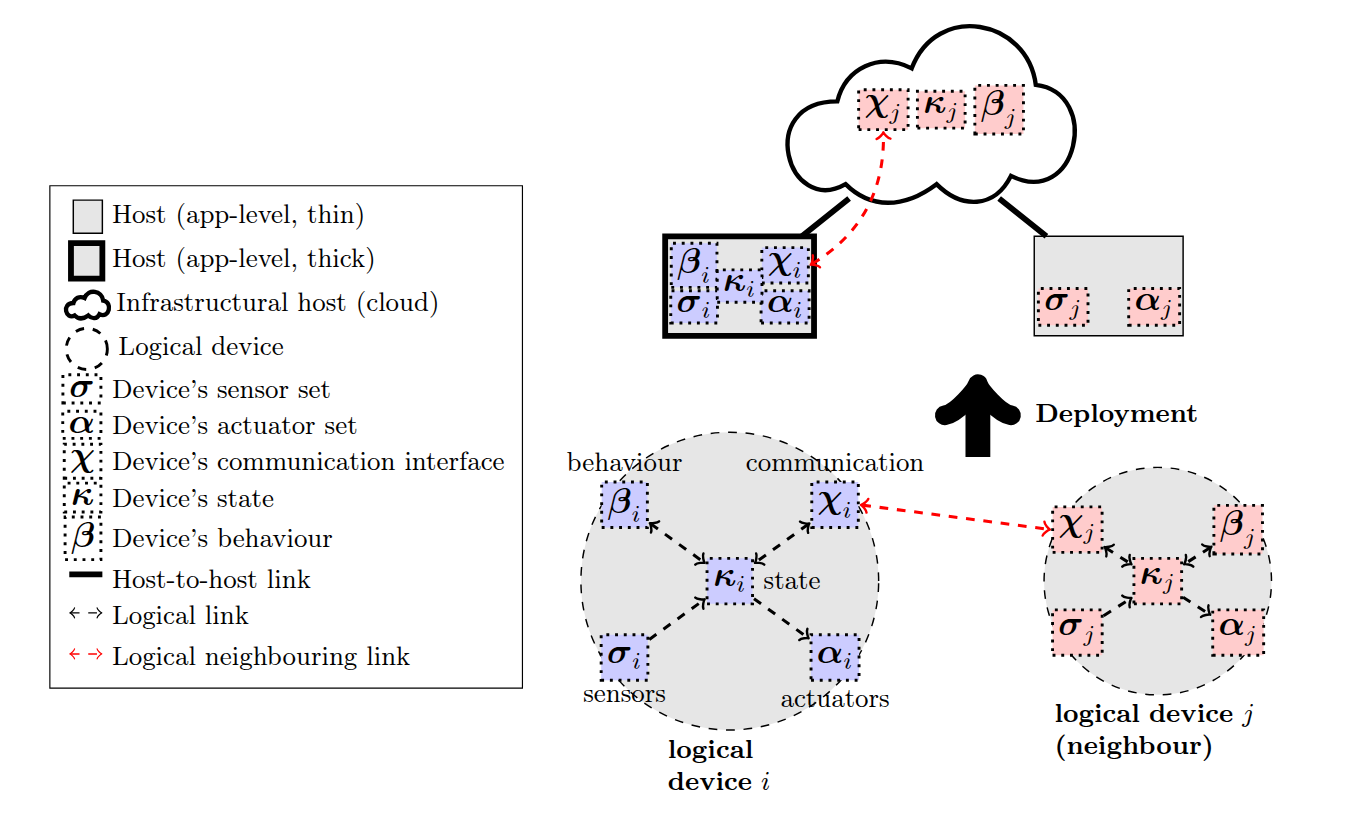
\includegraphics[width=\textwidth]{figures/image.png}
    \caption{Pulverization model for aggregate computing~\cite{DBLP:journals/fi/CasadeiPPVW20}.}
    \label{fig:pulverization-model}
\end{figure}

Each component can be deployed independently,
either on the same device or across different infrastructure nodes (e.g., edge, fog, or cloud servers).
%
This flexibility enables tailored deployments that balance energy efficiency,
latency,
and computational load.

For instance,
in a swarm robotics scenario,
robots with limited computational power can offload intensive processing tasks to more capable robots or cloud servers.
%
Meanwhile,
sensing and actuation components typically remain on the robots themselves.

Different deployment configurations,
such as fully peer-to-peer or fully cloud-based,
exhibit trade-offs in terms of latency, bandwidth consumption,
and energy usage.
%
Hybrid deployments,
where components are distributed across multiple devices,
offer opportunities to optimize these trade-offs.

\section{Research Activities and Outcomes}
\label{sec:research-activities}

My research activities started with a focus on the extension and development of approaches to foster \emph{deployment independence} of \ac{cas} in emergent and dynamic environments like the \ac{ecc},
and to support the system's reconfiguration at runtime.
%
In particular,
I've investigated dynamic reconfiguration aspects,
developing novel approaches and practical frameworks to support the relocation of pulverised components at runtime,
both from a pure local perspective (i.e., local reconfiguration rules) and from a global perspective (i.e., collective reconfiguration rules).
%
Relevant outcomes have been achieved in context where non-functional properties like cost,
power consumption,
and performance are optimized,
and the system's functional behavior is preserved.
%
This research has led to the publication and submission of several papers in high-quality journals and conferences,
as well as the development of new collaborations and research directions.

\subsection{Scientific Contributions and Activities}
\label{sec:scientific-contributions}

\subsubsection{Dynamic Deployment and Local Reconfiguration Policies}
At the beginning of my research,
I focused on developing innovative models to enhance the deployment independence of \ac{cas}.
%
Building upon previous work on pulverisation~\cite{DBLP:journals/fi/CasadeiPPVW20,DBLP:journals/iotj/CasadeiFPPSV22}---a modern approach to partition the execution model of CAS into independent components---I proposed a practical framework that implements and extends the pulverisation model to support dynamic components' relocation over the infrastructure at runtime.

To validate the proposed framework and the extended model with reconfiguration rules,
I conducted a series of experiments.
%
These experiments demonstrated the feasibility of the approach and highlighted its benefits in terms of deployment independence and non-functional properties,
such as cost,
power consumption,
and performance.
%
The results of this research have been published in a paper submitted to the \emph{Future Generation Computer Systems} journal~\cite{DBLP:journals/fgcs/FarabegoliPCV24}.

\subsubsection{Global Reconfiguration Policies and Load Balancing}
The limits exhibited by predefined reconfiguration rules in supporting the dynamic nature of \ac{cas} led me to explore a novel approach to better support the dynamic reconfiguration of \ac{cas} based on the pulverisation model.
%
Predefined reconfiguration rules may not be sufficient to cover all possible scenarios and may lead to suboptimal solutions,
such as oscillatory behaviors.
%
To address this issue,
I shifted the perspective from local reconfiguration rules to a global approach,
where the system's reconfiguration is expressed by a collective program leveraging \emph{Aggregate Computing}.
%
In this contribution,
I proposed a general pulverisation framework architecture where dynamic components' reconfiguration is treated as a first-class citizen and introduced a novel (collective) algorithm to balance the system's load during the reconfiguration process.

The proposed approach has been validated through a series of experiments,
demonstrating that the algorithm can better adapt to disruptive and changing conditions,
providing improved performance and stability compared to predefined allocations.
%
The results of this research have been published to the \emph{Internet of Things; Engineering Cyber Physical Human Systems} journal~\cite{DBLP:journals/iot/FarabegoliPCV24}.

\subsubsection{Extended Pulverized Model}
The pulverization model,
as presented in~\cite{DBLP:journals/fi/CasadeiPPVW20},
limits its partitioning system into only five components.
%
This coarse grained partitioning may not be desired or suitable for all applications,
especially when heterogeneous devices are involved.
%
For example,
robots or drones equipped with only microcontrollers may not sustain the entire \emph{behavior},
but only a slice of it.

Starting from this intuition,
we can identify in the macro-program functionalities requiring specific capabilities that may not be available on all devices.
%
To address this issue,
I proposed an orthogonal partitioning model allowing the system's specification to be defined in terms of ``wired'' independently deployable components (or functions).
%
In this model,
the macroprogram is specified as a direct-acyclic graph of interconnected components,
each representing a specific functionality of the system.
%
We further distinguish between \emph{local} components,
namely components not requiring interaction since they are merely transformation from input to output,
and \emph{collective} components,
which require interaction with other components instances belonging to neighbor devices to achieve the desired (collective) behavior.
%
This model can be seen as an orthogonal extension of the pulverization model,
achieving more flexibility and fine-grained partitioning.

Such a new model has been tested to proof its correctness in terms of functional correctness,
and its non-functional benefits in terms of power consumption in a wearable scenario.
Moreover,
a formalisation of the model has been provided through operational semantics,
and properties such as self-stabilisation preservation and deployment independence have been formally proven.
%
This work has been accepted and published at the \emph{Autonomic Computing and Self-Organizing Systems} conference~\cite{DBLP:conf/acsos/FarabegoliVC24}.

\subsubsection{AI-enhanced Pulverised Systems}

In the context of the \ac{ecc},
the dynamic nature of the infrastructure requires mechanisms for real-time resource management and system reconfiguration to maintain performance and efficiency under changing conditions.
%
To address this challenge,
I have explored the integration of AI-driven techniques,
such as reinforcement learning,
to enhance the dynamic reconfiguration of pulverised systems.
%
In this vision,
the system's reconfiguration is driven by an AI agent that learns optimal reconfiguration strategies through experience,
ensuring that the system adapts to changing conditions in real-time.
%
This research direction aims to optimize system performance and resource utilization,
while preserving the functional correctness of the system.

A preliminary study has been conducted investigating the combination of \ac{gnn} and \ac{rl} to support the relocation of pulverised systems.
%
In this study,
we formalised a general approach to support the dynamic component's relocation based on properties of the system and the infrastructure,
such as, but not limited to,
latency,
bandwidth,
and computational load.
%
This contribution has been accepted and presented at the \emph{Workshop ``From Objects to Agents'' 2024}~\cite{DBLP:conf/woa/DominiFAV24},
and at the PhD Symposium of the \emph{IEEE International Conference on Autonomic Computing and Self-Organizing Systems}~\cite{DBLP:conf/acsos/Farabegoli24}.

More consistent results are exercised in a subsequent work,
where a concrete toolchain has been proposed showing good benefits in terms of power consumption and performance.
%
This work has been submitted,
and it is currently under review to the \emph{ACM Transactions on Autonomous and Adaptive Systems}.

% Additionally,
% I developed a semi-formalisation of a novel approach to support the relocation of pulverisation components based on \ac{rl} and \ac{gnn}.
% %
% This vision aims to pave the way for intelligent \ac{cas} in modern infrastructures,
% where system reconfiguration is driven by AI-based techniques.

% An orthogonal contribution to the pulverisation model focused on partitioning the program specification of CAS into independent functions (or services) to achieve flexible deployment within the \emph{Edge-cloud Continuum}.
% %
% This approach aims to provide a more flexible and fine-grained system partitioning.
% %
% The proposed model has been formalised via operational semantics,
% with properties such as self-stabilisation preservation and deployment independence formally proven.
% %
% Experiments have shown that the approach preserves the functional behavior of the original monolithic system while offering non-functional benefits in terms of power consumption and performance, 
% with minimal communication overhead.
% %
% The results have been accepted and presented at the \emph{ACSOS 2024} conference~\cite{DBLP:conf/acsos/FarabegoliFAVE24}.

% Beyond my main research activities,
% I have collaborated with fellow PhD students and researchers on developing and evaluating coordination algorithms for UAVs and a novel federated learning approach.
% %
% These collaborative efforts have contributed to my research growth,
% expanding my knowledge and opening new research perspectives.

\subsection{Publications}
\label{sec:publications}

As a result of my research activities,
I've published and submitted the following papers:

\subsubsection{Accepted and Published}
\begin{refsection}[mypubblications.bib]
    % \DeclareFieldFormat{labelnumberwidth}{}
    \nocite{*} % Include all references from file1.bib only
    \printbibliography[heading=none]
\end{refsection}

\subsubsection{Submitted and Under Review}
\begin{enumerate}
    \item \fullcite{taas-heterognn} --- Submitted work and currently under review to \emph{ACM Transactions on Autonomous and Adaptive Systems} 
    \item \fullcite{coordination-prolog} --- Submitted work to \emph{COORDINATION 2025 -- International Conference on Coordination Models and Languages}
\end{enumerate}

% \begin{enumerate}

%     \item Nicolas Farabegoli, Danilo Pianini, Roberto Casadei, \& Mirko Viroli (2024). Scalability through Pulverisation: Declarative deployment reconfiguration at runtime. Future Gener. Comput. Syst., 161, 545–558.    
%     \item Farabegoli, N., Pianini, D., Casadei, R., \& Viroli, M. (2024). Dynamic Iot Deployment Reconfiguration: A Global-Level Self-Organisation Approach. Internet of Things Journal, Elsevier (submitted).
%     \item Davide Domini, Nicolas Farabegoli, Gianluca Aguzzi, \& Mirko Viroli (2024). Towards Intelligent Pulverized Systems: a Modern Approach for Edge-Cloud Services. In Proceedings of the 25th Workshop "From Objects to Agents", Bard (Aosta), Italy, July 8-10, 2024 (pp. 233–251). CEUR-WS.org.
%     \item Nicolas Farabegoli, Mirko Viroli, \& Roberto Casadei (2024). Flexible Self-organisation for the Cloud-Edge Continuum: a Macro-programming Approach. In IEEE International Conference on Autonomic Computing and Self-Organizing Systems, ACSOS 2024, Denmark, Aarhus, September 16-20, 2024. IEEE (to appear).
%     \item Denys Grushchak, Jenna Kline, Danilo Pianini, Nicolas Farabegoli, Martina Baiardi, Gianluca Aguzzi, \& Christopher Stewart (2024). Decentralized Multi-Drone Coordination for Wildlife Video Acquisition. In IEEE International Conference on Autonomic Computing and Self-Organizing Systems, ACSOS 2024, Denmark, Aarhus, September 16-20, 2024. IEEE (to appear).   
%     \item Davide Domini, Gianluca Aguzzi, Nicolas Farabegoli, Mirko Viroli, \& Lukas Esterle (2024). Opportunistic Fully-Distributed Federated Learning. In IEEE International Conference on Autonomic Computing and Self-Organizing Systems, ACSOS 2024, Denmark, Aarhus, September 16-20, 2024. IEEE (to appear).
%     \item Denys Grushchak, Jenna Kline, Danilo Pianini, \& Nicolas Farabegoli (2024). An Agent-based Model of Directional Multi-herds. In IEEE International Conference on Autonomic Computing and Self-Organizing Systems, ACSOS 2024, Denmark, Aarhus, September 16-20, 2024. IEEE (to appear).
%     \item Nicolas Farabegoli (2024). Intelligent Pulverised Collective-adaptive Systems. In IEEE International Conference on Autonomic Computing and Self-Organizing Systems, ACSOS 2024, Denmark, Aarhus, September 16-20, 2024. IEEE (to appear).
% \end{enumerate}

\subsection{Conferences and Workshops}

During this first year of my PhD,
I've attended the following conferences and workshops:

\begin{itemize}
    \item Attended the \emph{International ABS Workshop 2023};
    \item Presented a paper at the \emph{Workshop ``From Objects to Agents'' 2024};
    \item Attended \emph{ACM SIGPLAN International Conference on Functional Programming};
    \item Presented 2 out of 5 papers at the \emph{IEEE International Conference on Autonomic Computing and Self-Organizing Systems - ACSOS 2024}.
\end{itemize}

% \subsection{Research Goals}

% \subsection{Literature Review}

% \section{Academic Activities}

% \subsection{Tutoring Activities}

% In this first year of my PhD,
% I have been involved in tutoring activities for the course \textbf{PROGRAMMAZIONE AD OGGETTI [cod. 70219]} for the Bachelor's Degree in Computer Science and Engineering for the academic year 2023/2024,
% and currently involved in the academic year 2024/2025 edition of the same course.

% \subsection{Doctoral School and Courses}

% I've attended the \textbf{Bertinoro International Spring School 2024} in March 2024,
% in particular I've attended the \emph{Graph Neural Network} course by Prof. Fabrizio Silvestri,
% the \emph{Program analysis: from proving correctness to proving incorrectness} course by Prof. Roberto Bruni and Robera Gori,
% and the \emph{Large Language Models} course by Prof. Danilo Croce.
% %
% Moreover,
% I've attended the following PhD courses:
% \begin{enumerate}
%     \item \emph{How to Write and Publish a Research Paper in Computer Science and Engineering} by Prof. Zeynep Kiziltan;
%     \item \emph{Risk Assessment of Machine Learning for Cybersecurity} by Prof. Fabio Pierazzi;
%     \item \emph{Introduction to complex systems science} by Prof. Andrea Roli;
% \end{enumerate}
% At the end of the first year,
% I've obtained \textbf{15} CFU with evaluation, and \textbf{4} CFU without evaluation.

% \section{Self Evaluation}

% I strongly believe that the first year of my PhD has been very productive and successful.
% %
% Despite initial difficulties in getting my works accepted in conferences and journals,
% I've been able to publish and submit three papers in high-quality venues,
% and I've been able to collaborate with other researchers and PhD students in different research areas.
% %
% During this year,
% I've been able to improve my research skills,
% and I've been able to learn new techniques and methodologies to address research problems,
% get familiar with new research tools and environments,
% and improve my writing and presentation skills.

\section{Research Roadmap}
\label{sec:future-directions}
As follows,
a tentative roadmap for the next years of my PhD is presented.
%
The roadmap is divided into three main research directions: \emph{Models},
\emph{Deployment Platforms},
and \emph{Dynamic Reconfiguration}.

\subsection{Models}
Even though the pulverisation model has been extended to support more flexible and fine-grained partitioning,
future research must focus on how this model can be applied not only to aggregate computing,
but more in general,
to collective systems.
%
This goal requires a deep investigation of the model's properties,
providing general abstractions that can be reused across different paradigms for implementing collective systems.

\subsection{Deployment Platforms}
The actual gap between simulation and real deployment of pulverised systems must be addressed.
%
A preliminary toolchain has been developed to support the deployment of pulverised systems~\cite{DBLP:journals/fgcs/FarabegoliPCV24,DBLP:conf/acsos/FarabegoliVC24},
but a more general,
comprehensive framework is needed to close the gap between simulation and real deployment.
%
The focus of this research direction is to provide a
flexible platform supporting the entire engineering process from its conceptualization,
its design,
its simulation in a controlled environment,
up to its deployment in the real world.
%
An intriguing investigation must involve the adoption of multitier programming~\cite{DBLP:journals/pacmpl/WeisenburgerKS18},
since it has common similarities with macroprogramming~\cite{DBLP:journals/csur/Casadei23} models,
where distributed systems are defined in a single program,
but differently from aggregate computing,
for instance,
the focus is on the soundness of the communication among the tiers of an infrastructure,
key aspects when dealing with the \ac{ecc}.
%
Even if this platform is supposed to be general,
I plan to use aggregate computing as a case study to validate the platform.

\subsection{Cross-language Support}
Device heterogeneity force the adoption of diverse technological stacks,
and consequently,
different SDK and programming language.
%
Base on works like~\cite{DBLP:journals/jss/BertolottiCOC24},
which do not directly apply the approach to distributed systems,
I will investigare a ``common'' core of the platform that can be ``reified'' into different platforms,
enabling a seamless interoperability among different devices and programming languages.
%
This direction will be a pillar for managing the heterogeneity of the \ac{ecc}.

\subsection{Dynamic Reconfiguration}
Dynamic relocation and deployments have covered a significant part of my research activities~\cite{DBLP:journals/fgcs/FarabegoliPCV24,DBLP:journals/iot/FarabegoliPCV24}
%
However,
dealing with a high number of devices,
unpredictable changing conditions such as network latency,
bandwidth,
and computational load,
requires more advanced techniques to support the system's reconfiguration.
%
A preliminary study has been conducted and presented in~\cite{DBLP:conf/woa/DominiFAV24},
but a more deep investigation is needed to provide a comprehensive framework to support the dynamic reconfiguration of pulverised systems,
as presented in the previous sections.
%
In this context,
I will investigate how to devise a general AI-based reconfiguration model supporting dynamic deployments,
that integrates with the high-level programming models proposed as a future research direction.
%
In particular,
I aim to investigate how capabilities can permeate from the design to the reconfiguration,
ensuring safety and correctness of the system at runtime.

% I plan to continue my research on developing innovative models for engineering collective adaptive systems.
% %
% My focus will be on integrating techniques that support comprehensive
% and effective reconfiguration strategies while exploring multitier programming~\cite{DBLP:journals/csur/WeisenburgerWS20} models to facilitate the deployment of collective systems in the \ac{ecc}.
% %
% In this context,
% I aim to investigate the use of capability-based mechanisms for controlling system deployment and runtime reconfiguration,
% ensuring that system specifications are correct by construction leveraging advanced type systems.
% %
% Additionally,
% I am interested in integrating AI-based techniques to support runtime reconfiguration while preserving the functional correctness of the system,
% ensured at the design time by the type system.


%
% ---- Bibliography ----
%
% BibTeX users should specify bibliography style 'splncs04'.
% References will then be sorted and formatted in the correct style.
%
% \nocite{*}
% \bibliographystyle{splncs04}
% \bibliography{bibliography,mypubblications}
\printbibliography

\end{document}
